\documentclass[a4paper, 12pt]{article}

\usepackage[portuges]{babel}
\usepackage[utf8]{inputenc}
\usepackage{amsmath}
\usepackage{indentfirst}
\usepackage{graphicx}
\usepackage{multicol,lipsum}

\begin{document}

\begin{titlepage}
    \begin{center}

        \begin{figure}[!ht]
            \centering
            
\includegraphics[width=10cm]{images/IST.png}
        \end{figure}

        \Huge{Instituto Superior Técnico}\\
        \large{LEEC}\\
        \large{Sinais e Sistemas}\\
        \vspace{15pt}
        \vspace{95pt}
        \textbf{\LARGE{Relatório Laboratório Sinais e Sistemas}}\\
        \vspace{3,5cm}
    \end{center}

    \begin{flushleft}
        \begin{tabbing}
            Aluno: Henrique Machado 103202 \\
            Aluno: Miguel Neves 103462 \\
        \end{tabbing}
    \end{flushleft}
    \vspace{1cm}

    \begin{center}
        \vspace{\fill}
        Janeiro\\
        2023
    \end{center}
\end{titlepage}
%%%%%%%%%%%%%%%%%%%%%%%%%%%%%%%%%%%%%%%%%%%%%%%%%%%%%%%%%%%
% % % % % % % % % % % % % % % % % % % % % % % % % %
\newpage
\tableofcontents
\thispagestyle{empty}
\newpage
\pagenumbering{arabic}
% % % % % % % % % % % % % % % % % % % % % % % % % % %
\section{Sinais Sinusoidais}
\begin{itemize}
    \item \textbf{Q1:} As sinusoidais com frequência mais altas correspondem aos sons mais graves, inversamente, as sinusoidais com frequência mais baixa correspondem aos sons mais graves.
    \item \textbf{Q2:} A frequência minima que nós conseguimos ouvir foi $55hz$ e a frequência máxima que conseguimos ouvir foi $18000hz$.
\end{itemize}
% % % % % % % % % % % % % % % % % % % % % % % % % % %
\vspace{15px}
\section{Notas Musicais}
\begin{itemize}
    \item \textbf{Q3:}
          \begin{enumerate}
              \item[] Mi$_4$: $329.63hz$
              \item[] Fá$_4^\#$: $370.00hz$
              \item[] Sol$_4$: $392.00hz$
              \item[] Si$_4$: $493.89hz$
              \item[] Dó$_5$: $554.37hz$
          \end{enumerate}
\end{itemize}
% % % % % % % % % % % % % % % % % % % % % % % % % % %
\vspace{15px}
\section{Impulso e Degrau Unitários}
\begin{itemize}
    \item \textbf{Q4:} Com base na definição de degrau unitário, $u(at+b)$ pode ser escrito como $u(\pm t - t_0)$ uma vez que: $t_0 = \frac{b}{|a|}$, onde temos que
    \[ \begin{cases} 
      a > 0, & t > 0\\
      a < 0, & t < 0
    \end{cases} \]
    Caso $a < 0$, verifica-se uma inversão no tempo do gráfico de $u(t)$.
    \newpage
    \item \textbf{Q5:} $\delta(at) = \frac{1}{\Delta}[u(at) - u(at - \Delta)]$ e $\delta(at) = \underset{{\Delta\to0}}{\lim}\delta_\Delta(at)$, com $a > 0$\vspace{15px}\\
    Para $\delta(t)$\hspace{150px}Para$\delta(at)$\\
    \begin{figure}[!ht]
        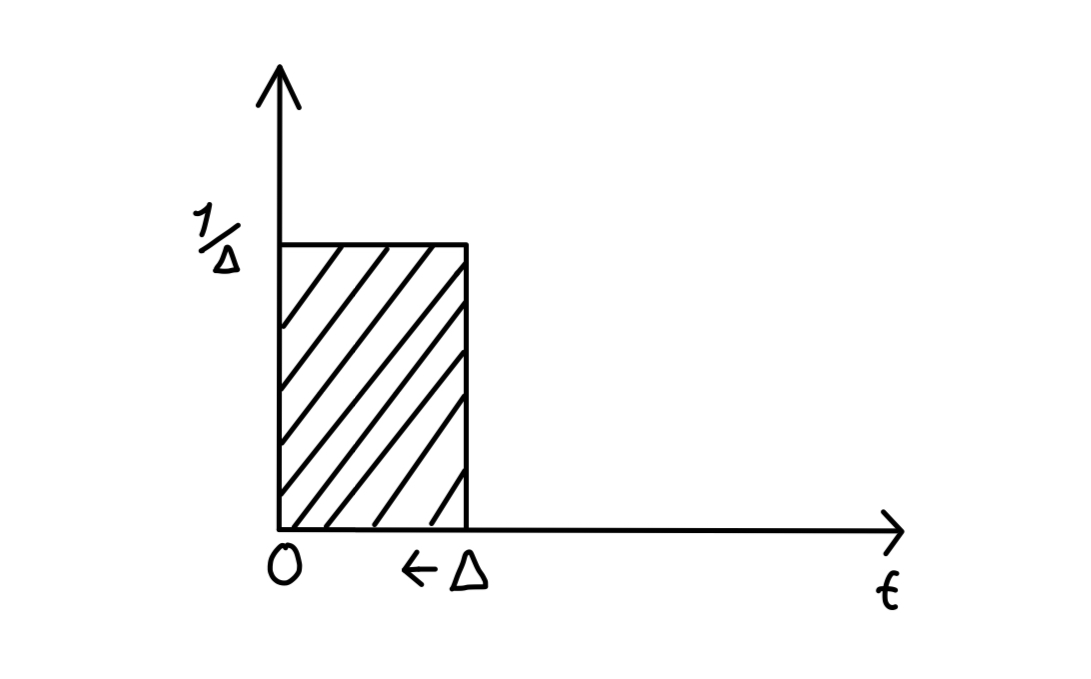
\includegraphics[width=6cm]{images/Graf1.png}
        \hspace{10px}
        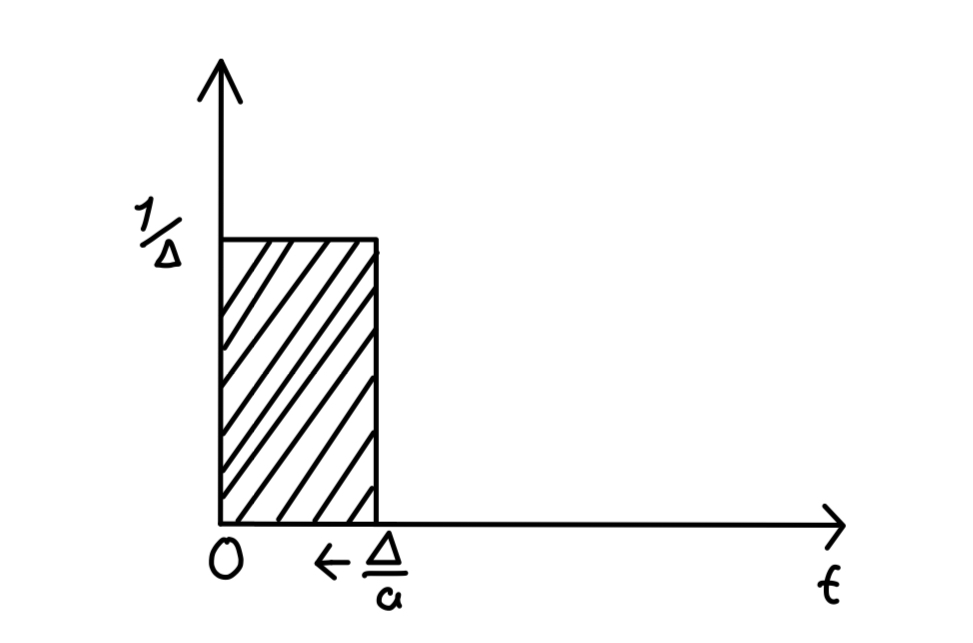
\includegraphics[width=6cm]{images/Graf2.png}
    \end{figure}\\
    Área $ = \frac{1}{\Delta}\times\Delta = 1$\hspace{100px}Área $= \frac{1}{\Delta} \times \frac{\Delta}{a} = \frac{1}{a}$\vspace{15px}\\
    Logo, $\delta(at) = \frac{1}{a}$, com $a > 0$.\vspace{5px}
    \item \textbf{Q6:} Pela visualização do gráfico de $\delta(at)$, não se verificam alterações em relação ao gráfico de $\delta(t)$, o que não está correto. O escalamento deveria.
\end{itemize}
\newpage
% % % % % % % % % % % % % % % % % % % % % % % % % % %
\section{Sistemas}
\newpage
% % % % % % % % % % % % % % % % % % % % % % % % % % %
\section{Série de Fourier}
\newpage
% % % % % % % % % % % % % % % % % % % % % % % % % % %
\section{Resposta em Frequência}
\newpage
% % % % % % % % % % % % % % % % % % % % % % % % % % %
\section{Filtragem}
\newpage
% % % % % % % % % % % % % % % % % % % % % % % % % % %
\section{Amostragem}
% % % % % % % % % % % % % % % % % % % % % % % % % % %
\end{document}